% Dynamic optimisation project proposal
% J Brown 2003,2004

\documentclass[11pt,letterpaper,onecolumn,notitlepage]{article}

% \setlength{\columnsep}{8mm}

\usepackage{verbatim}
% \usepackage{fancyhdr}
\usepackage{ltxtable}
\usepackage{amssymb}
% \usepackage{doublespace}
\usepackage{hyperref}
\usepackage{times}                      % use times
% \renewcommand{\ttdefault}{cmtt}         % but don't use courier for typewriter

\DeclareMathAlphabet{\mathsl}{OT1}{ppl}{m}{s}

\usepackage{graphics}			% to allow postscript inclusions

\input{epsf}				% to allow postscript inclusions
% On thor and CUS read top of file:
%     /opt/TeX/lib/texmf/tex/dvips/epsf.sty
% On CL machines read:
%     /usr/lib/tex/macros/dvips/epsf.tex



\raggedbottom				% try to avoid widows and orphans
\sloppy
\clubpenalty1000%
\widowpenalty1000%

% \addtolength{\oddsidemargin}{6mm}	% adjust margins
% \addtolength{\evensidemargin}{-8mm}

% \renewcommand{\baselinestretch}{1.5}	% doublespace

\setlength{\parskip}{1.5ex}
\setlength{\parindent}{0pt}

\begin{document}

\title{Dynamic Optimisation}
\author{Julian Brown (brown@cs.bris.ac.uk)}
\maketitle

\bibliographystyle{plain}


\newenvironment{code}
  {\begin{list}{}{
    \setlength{\rightmargin}{\leftmargin}
    \raggedright
    \setlength{\itemsep}{0pt}
    \setlength{\parsep}{0pt}
    \ttfamily}%
   \item[]}
  {\end{list}}


%%%%%%%%%%%%%%%%%%%%%%%%%%%%%%%%%%%%%%%%%%%%%%%%%%%%%%%%%%%%%%%%%%%%%%%%%%%%%%
% Title


% \pagestyle{empty}

% \include{title}

% \cleardoublepage

\cleardoublepage	% just to make sure before the page numbering
			% is changed

%\setcounter{page}{1}
%\pagenumbering{arabic}
%\pagestyle{headings}

\section{Background and motivation}

The first widely-used optimising compiler was IBM's 1957 Fortran I compiler, whose code generation ability remained unparallelled for the next 20 years. This work pioneered many important optimisation techniques which are now used by virtually all compilers: copy propagation, dead-code elimination, strength reduction and register allocation. It also demonstrated precursors to several other techniques.

Since then, compiler technology has improved very slowly, in contrast to the improvements seen in CPU technology. The often-quoted (though perhaps inaccurate) statistic that CPU power doubles every 18 months is reflected by Todd Proebsting, stating ``compiler technology doubles CPU power every 18 {\em years}'' \footnote{emphasis mine}.

Furthermore, techniques and idioms are available to programmers now, such as abstract data types, virtual functions, data hiding (with accessor methods), higher-order functions and iterators which sacrifice the efficacy of even the traditional compiler optimisations in favour of development speed, correctness of programs, portability and expressive power. Also for pragmatic reasons, such as code sharing between projects or the practice of distributing patches, plugins or applets over the internet, large desktop applications are written not as monolithic entities but as collections of shared libraries. While convenient, this unfortunately negates the possibility of doing any whole-program optimisation.

To obtain performance beyond the four-fold increase an optimiser is likely to provide, code must be manually optimised by the programmer. To quote Michael Abrash, ``the best optimiser is the one between your ears''. If a programmer needs to make a program run faster, perhaps the worst thing he has to do is break his carefully thought-out abstractions, because their overheads are too high. Advances in software engineering are, by and large, a good thing: a programmer should be free to use abstract data types, for example, with the reassurance that they will be executed as efficiently as native data types (for languages which make the distinction, anyway). Likewise, a call to a function or method in a shared library, perhaps even one which was originally written in a different language, should be as fast as a call to a function defined in the same module. If this is the case, a programmer can concentrate on making his code correct, easy to understand and maintainable rather than just making it fast at the expense of all else.

We are working on the hypothesis that traditional optimisation is limited because a compiler typically knows nothing, or very little, about how a program is going to behave when it is executed. By this we mean where it spends most of its execution time, where it does lots of memory accesses, whether conditional branches are taken or not taken, which functions are executed frequently and so on. The compiler must make many thousands of decisions when compiling a given program based on heuristics tuned to the ``average case'', whereas the code in question might exhibit significantly different characteristics.

A typical solution to this problem is a combination of whole-program optimisation and feedback-directed optimisation. The former adds the capability to the compiler of considering more than one source code file simultaneously during optimisation phases, and the latter requires compilation with profiling enabled, a run of the program with a body of ``typical'' data, and then re-compilation guided by the data gathered during the run. This is obviously inconvenient, and will slow down the program's development cycle.

Even in the case where the compiler supports whole-program optimisation and feedback-directed optimisation, if the program links to any libraries -- static or shared -- we probably won't have access to all their source code too, limiting the scope of our optimisations to within our own source tree. Often library source code is proprietary, so there isn't even a chance to incorporate critical sections into our code.

We aim to investigate an alternative strategy, which moves the burden of optimisation away from the compiler and onto a support layer in the run-time system. Our optimisations should be language-independent and will work in the absence of source code. Since binary code is not well suited to analysis and re-optimisation, we will design and implement a system from the ground up which is better tuned to supporting the type of operations we want to do.

Using run-time optimisation will enable us to determine how a program is executing at a given point in time, and so open the opportunity to create an improved or specialised version of the code given that information. We can then rewrite the program binary on-the-fly so that it will execute more efficiently.

Starting from the following section, we will define what we mean by dynamic optimisation, then look at existing work in this field, then we will discuss the work we plan to do in this area. We finish with a work-plan broken down into milestones detailing the research we intend to carry out.

\section{Optimise for what?}

It is best to start out by defining what we mean when we say optimisation. There are several factors for which it might be meaningful to optimise:

\begin{itemize}
\item Speed
  \begin{itemize}
  \item Number of instructions
  \item Number of cycles
  \item Number of data/instruction cache misses
  \item Number of page faults
  \end{itemize}
\item Space
  \begin{itemize}
  \item In permanent storage (or over a network)
  \item Whilst running
  \end{itemize}
\item Power consumption
\end{itemize}

Ideally, we would want compiler optimisations to make generated code both smaller and faster, but these two goals are contradictory to some extent. Optimising for speed will often increase program size, and optimising for size might lead to slower code execution. In some cases though, smaller code may exhibit a higher code-cache hit rate, which could improve the program's performance!

Our optimisation criterion also depends on the type of system our code will be running on. On a desktop PC, memory is now cheap and plentiful, but that might not be the case on a smaller device such as a PDA or cellphone. So for a desktop PC, we are likely to want to optimise for speed at the expense of space, but for a smaller system it is likely that we will want to optimise for size over speed.

When optimising for space, we are referring to the `compactness' of generated code only, not to anything else (eg the heap size of the running program). More aggressive optimisations might duplicate code, for instance by unrolling loops or inlining larger functions. These techniques not only remove the overhead of branches (loops) or calls (functions), but can also improve instruction scheduling on superscalar processors. However if space is at a premium, as little code as possible should be duplicated. Dynamic optimisation is not likely to become a good technique for reducing the size of running programs, but program binaries could become smaller by deferring loop unrolling and function inlining until run-time. This would be particularly relevant if transferring binaries over slow or expensive network connections, without impacting their overall performance.

Measuring speed optimisations can be complicated, especially if we are running on a system with multiple caches, virtual memory, multiple concurrent processes and out-of-order instruction scheduling. If we add a dynamic optimisation system to the run-time environment of a program, we factor in yet another layer of complexity. We are interested in the total time a program takes to run, and it is this which we aim to reduce even when running our optimisation system at the same time. Since we are not going to be building real hardware, this should be shown in a realistic simulated environment.

Optimising for power consumption is a fairly new topic and will become increasingly important as more sophisticated code is run on handheld computers and other small devices. Dynamic optimisation provides some interesting possibilities for power optimisation too -- we will revisit this idea later on in this document.

Existing work related to dynamic optimisation work has already shown promising results for both size optimisation \cite{AdaptCtxInline} and speed optimisation \cite{Deco,Dynamo,WigginsRedstone,Mojo}, but success has been limited by working on legacy architectures. We hope that since our instruction set and support hardware will be more suited to dynamic optimisation, we will be able to achieve better results.

\section{Hypothesis}

We assert that a dynamic optimisation system can do better at optimising code than a static optimising compiler. We base this claim on three observations. The first is that the `trace' of {\em dynamic} instructions entering a processor typically looks fairly bloated and redundant if viewed sequentially, even for quite highly-optimised code. The second is that, with a dynamic optimisation system, we should be able to adapt a program to the data it is actually working on at any given point, which might vary during its execution.

The third observation is one which is cited often, that a program spends 90\% of execution time in just 10\% of its code (an instance of Zipf's Law). This weighting can be seen in figure \ref{gzipfreq}, made using an early version of our toolchain, which represents the frequencies of transitions between pairs of basic blocks recurring more than 100 times during the compression of a small file with the {\tt gzip} program. This observation is what makes dynamic optimisation feasible, since not all of an executable program's code needs to be processed, only those parts which are executed most frequently.

Existing research has shown that purely software-based dynamic optimisation systems are capable of improving the performance of compiled binary code, even when it has already been highly optimised statically \cite{Dynamo}. However, many of the existing systems are limited by bottlenecks which cannot easily be removed whilst working with the same hardware. We hope to show that a system designed specifically to optimise code as it is executing, using a hybrid hardware/software approach, would be able to improve the performance of a large range of programs substantially beyond the existing work in the field.

\begin{figure}[t]
\centerline{\rotatebox{-90}{\scalebox{0.5}{
\includegraphics{gzipfreq.ps}
}}}
\caption{\label{gzipfreq}Execution of gzip on a small file}
\end{figure}

\section{Existing work}

\subsection{Processor architecture}

Many techniques employed by modern CPUs already employ techniques which can be thought of as dynamic optimisation. Caches are filled according to the flow of code and data at runtime, and register renaming is also dependent on which code is executed. Branch prediction attempts, with a high success rate, to guess which way a conditional branch will go, based on the outcome of earlier conditional branches.

Out-of-order execution of instructions enables a processor to occupy its functional units depending on the dynamic stream of instructions which flow into it. Systems which attempt to multiply-dispatch instructions based on static scheduling (eg, Intel's IA-64 architecture) have been somewhat less successful, since then all instruction-level parallelism must be extracted from the code using complex data-flow analyses, which as yet have not advanced sufficiently to catch up with the dynamic approach. Even when good enough compilation algorithms have been developed, code expansion because of necessary redundancy will still be a problem.

Intel's Pentium 4 core contains a ``trace cache'', which is reminiscent of the traces used by Dynamo \cite{Dynamo}, and by similar and derivative works. More recent Pentium 4 cores employ a technique named ``hyperthreading'', which is able to dispatch instructions from a second execution thread whilst the first is blocked on a memory access. Both of these techniques are exploiting dynamic usage patterns to increase the throughput of the processor.

IBM's research project BOA (Binary-translation Optimised Architecture) and Sun's MAJC (Microprocessor Architecture for Java Computing) both touch on ideas that I am presenting here. BOA utilises code translation as a way of executing PowerPC code at very high clock rates, and MAJC is designed to be a good target for high-performance Just-In-Time (JIT) compilation, the eventual aim being to make software independent from particular instruction sets, and eliminate binary compatibility issues.

\subsection{Dynamic optimisation systems}

The canonical reference for dynamic optimisation systems is Hewlett Packard's research project Dynamo \cite{Dynamo}. Dynamo is able to improve the performance of native PA-RISC binaries through a combination of an interpretive emulator, a very low-overhead hot trace profiling method, and a software-based optimiser. Dynamo is able to boost the performance of binaries compiled with the {\tt -O2} optimisation level (with HP's compiler) to the same performance as the equivalent {\tt -O4} binaries. This is especially interesting because this performance is achieved {\em despite} running programs through emulation, though it is mostly effective only on programs which run for more than two minutes. Dynamo has since been extended to run on other architectures, and serves as the basis for several other projects (DynamoRIO, DO \cite{KimHazelwood}). Other projects include Deco \cite{Deco}, Mojo \cite{Mojo} and Wiggins/Redstone \cite{WigginsRedstone}.

\subsection{Language-specific work}

Many techniques which may be useful for dynamic optimisation systems were pioneered by the virtual machines for various language implementations. Smalltalk, and latterly Java, use JIT compilation to speed up execution of bytecodes. This technique is a specialised form of dynamic optimisation, where the flow of execution of the code which interprets each bytecode is `optimised' into contiguous native code fragments based on its data -- the Java/Smalltalk program.

The Jalape\~{n}o/Jikes virtual machine \cite{Jalapeno} adds dynamic compilation and adaptive optimisation to Java, giving further performance improvements.

A project named Fabius \cite{Fabius} adds dynamic compilation support to ML, generating specialised versions of functions when curried functions are partially applied, leading to 600\% speed increases in some benchmarks.

Dawson Engler and others developed `C (tick-C) \cite{tcc}, a language which enriches C with support for run-time compilation of code. Although programmer intervention is required, performance increases of up to an order of magnitude were achieved over the statically-compiled equivalent code using their prototype compiler {\tt tcc}.

R. G. Burger's Ph.D. thesis \cite{DoScheme} describes extensions to a Scheme run-time environment which adds intraprocedural register allocation and profile-driven dynamic recompilation. In the conclusion, he claims that around 72\% of stack accesses can be eliminated through the mechanism he describes, and run-time performance increases by around 43\% when six registers are available for parameters and local variables.

\section{Work plan}

\subsection{The challenge}

We feel that the work to date in this area has barely scratched the surface of what should be possible with dynamic optimisation. We have already built a considerable amount of the infrastructure necessary to perform research in this field. We have an instruction-set architecture (ISA), simulator, compiler tools (including a port of the GCC compiler) and the beginnings of a software-based optimisation system. The challenge is making a system which is simple enough to have a chance of being demonstrably correct, but which is at the same time sophisticated enough to demonstrate real benefits from the techniques we develop.

As such, our ISA is tuned not only to be easy to execute using hardware, but also easy to decode in software and with clean, straightforward semantics so that higher-level representations can be inferred and manipulated very quickly. By starting with a clean slate, we not only avoid the cruft present in many existing architectures, but we are able to make fundamental changes in areas such as code layout and control flow. Our ISA also contains hints for the optimiser passed down through the compiler toolchain, so more information is available at run-time than with most existing architectures. Because code will be modified dynamically rather frequently, there is a mechanism which allows us to replace sections of code much more efficiently than traditional architectures would allow.

Profiling of code is very important, and has been the main bottleneck for several extant projects. We anticipate moving the burden of profiling the execution of code onto hardware. Various profiling strategies might have different hardware or performance costs, so we will build models to investigate what works and what doesn't.

Our work will involve the design of algorithms for partial decompilation, specialisation of binary code, optimisation, code generation and management of optimised code. Because these algorithms must run in real time, it is important that they are highly efficient. Many existing compiler techniques may have to be modified or disregarded if they take too long to execute. 

We hope to investigate the possibility of automatically specialising code based on variables which turn out to be constants -- or `almost' constants -- at run time. This would mean that conditional branches could be deconditionalised, arithmetic operations simplified, and larger `straight-line' blocks of code could be created, which are the most amenable to caching, prefetch insertion and speculative execution on modern processors. No existing dynamic optimisation systems that we are aware of are able to pro-actively detect constants and rewrite code in this way.

The literature is lacking in information about what kinds of optimisations can be done within a dynamic framework, where there is a tradeoff concerning time spent optimising a program being time spent not running that program. Work in this area could have a direct impact on the design of virtual machines for conventional programming languages, even on existing hardware.

Also uninvestigated by dynamic optimisation research is code which needs to meet real-time constraints (eg, multimedia applications), and still be optimised. Altering the parameters of our simulations should allow us to investigate the possibility of using ``slave'' coprocessors specifically for optimising the code of the main processor without interrupting program execution. We are not aware of any existing data about how well such a coprocessor would work in practice.

Power consumption optimisations would also be possible using the same techniques we are developing, for example we could disable parts of the CPU (eg, multiplication or division units) when in a low-power mode, rewriting code by synthesising alternate code sequences or library calls in place of the power-hungry instructions. This would mean that code could still run, but in a reduced capacity. When full power returns, the original code stream could be restored along with the disabled CPU units.

\subsection{Milestone 1}

Coarse simulation of simple binaries. Development of profiling algorithms suitable for hardware implementation. Hand-analysis of code. Robust identity transform in optimiser (via an intermediate representation).

\subsection{Milestone 2}

Automatic dispatch of optimiser based on profile data. Simple optimisations (block merging, constant propagation, copy propagation, branch deconditionalising).

\subsection{Milestone 3}

Accurate simulation, including cycle-accurate processor, cache and memory system emulation with a core supporting out-of-order execution. Instruction scheduling optimisations. Profiling for data-dependent specialisation.

\subsection{Milestone 4}

Specialisation-based optimisations. Demonstration of beneficial effects on SPEC benchmarks.

\section{Funding and benefit to funding body}

The first three years of this work were funded by an EPSRC studentship, which has now expired. The current status of the project is as follows. We have an instruction set, an instruction-set simulator and a compiler toolchain including a port of the GNU C compiler (GCC). Parts of milestones 1 and 2 (the dynamic optimiser proper) are complete: we can recover clean abstract code trees from binary code fragments, manipulate them and translate them back into binary code without loss of information or code quality. As such the work is at a critical stage: much more needs to be done before it can be turned into a Ph.D., but it has now reached the stage where interesting research can begin.

However, we need additional funding to complete this work. We are also seeking industrial collaborators who are able to offer feedback, or perhaps code samples they would like to be optimised using this sort of technique in the future.

This work will not directly benefit the general public. We aim to investigate an area of computer architecture which might not seem suitable for a commercial product due to its high-risk nature, but which may provide high rewards if experiments turn out to be successful.

A processor built around this type of architecture would provide benefits for fringe programming languages or compilers, which could leverage the optimisations provided by our run-time system to avoid needing a full-blown optimiser themselves. Virtual machines which themselves generate code on-the-fly (eg Java) could equally benefit, since their code must be generated very quickly so is probably not very optimal to start with.

Families of processors built around this type of architecture would be immune both to issues of binary incompatibility, and legacy code optimised for a particular implementation of an architecture. In the former case new instructions could be synthesised by the optimisation layer into sequences of old instructions, and in the latter case code can be reoptimised for a different architecture implementation.

Please contact Julian Brown ({\tt brown@cs.bris.ac.uk}) for further information.


%%%%%%%%%%%%%%%%%%%%%%%%%%%%%%%%%%%%%%%%%%%%%%%%%%%%%%%%%%%%%%%%%%%%%%%%%%%%%%
% the bibliography

% \addcontentsline{toc}{chapter}{Bibliography}
\bibliography{refs}
% \cleardoublepage

%%%%%%%%%%%%%%%%%%%%%%%%%%%%%%%%%%%%%%%%%%%%%%%%%%%%%%%%%%%%%%%%%%%%%%%%%%%%%%
% the appendices
% \appendix

\end{document}
